\documentclass[12pt,english]{scrartcl}

\usepackage{amsmath,amsfonts,amssymb,amscd,amsthm,amsbsy,alltt,bera,upref,fancyvrb}
\usepackage[T1]{fontenc}
\usepackage{babel}
\usepackage{graphicx}
\usepackage{tikz}

\textheight=10.0truein
\textwidth=6.8truein
\hoffset=-.5truein
\voffset=-.5truein
\pagestyle{headings}
\footskip=36pt
\swapnumbers
\DefineVerbatimEnvironment{code}{Verbatim}{fontsize=\small}
\DefineVerbatimEnvironment{example}{Verbatim}{fontsize=\small}

\usepackage{xcolor}
\definecolor{shade}{RGB}{240,255,255}
\definecolor{nw}{RGB}{255,239,213}

\makeatletter
    \setkomafont{section}{\color{white}%
        \bfseries\Large
        
\begin{tikzpicture}[overlay]
        \draw[fill=black] (0,-2pt) rectangle
        (\linewidth,16.4pt);
        \end{tikzpicture}}
    \setkomafont{subsection}{\color{black}%
        \bfseries\Large
        \begin{tikzpicture}[overlay]
        \draw[fill=white] (0,-2pt) rectangle
        (\linewidth,16.4pt);
        \end{tikzpicture}}

\def\and{%
  \end{tabular}%
  \hskip 1em \@plus.10fil\relax
  \begin{tabular}[t]{c}}
\makeatother
\makeindex

\title{Technical Report: The Austinites}
\author{
  Sheeyla Garcia\\
  \and
  Jesus Hernandez\\
  \and
  Kyle Nicola\\
  \and
  Stephen Ridings\\
  \and
  Carlos Rodriguez\\
  \and
  Mark Sandan\\  
}
\date{ July 24, 2014 }
\begin{document}
\thispagestyle{plain}
\maketitle
\tableofcontents

\begin{figure}[h!]
\includegraphics[width=\textwidth]{homev2}
 \caption{Splash Page for the second iteration of IDB2 showing the group name and the buttons in the three main pages.}
\end{figure}

\section{Updates}
Updates for the second iteration at a glance:
\begin{itemize}
 \item the splash page and web design has been $fancied up$ 
\end{itemize}
\begin{itemize}
 \item Dynamic webpages supporting our models instead of static webpages
\end{itemize}
\begin{itemize}
 \item MySQL is being used currently as the database backend
\end{itemize}
\begin{itemize}
 \item Django Rest framework installed to implement the API
\end{itemize}
\begin{itemize}
 \item Refactored the Models used to include a Media models. Photo and Member models have been deprecated.
\end{itemize}
\begin{itemize}
 \item Django commands have been installed to load data from formatted text files for Artist, Stage, and Sponsor
\end{itemize}

\subsection{Summary}
The main changes that have been made can be summarized into three categories: dynamic functionality, REST implementation, and the model refactoring. 

To implement a dynamic webpage we are currently using html,css,javascript, and the django template language to access instances of Artists, Sponsors, and Stages to fill the content of the webpages. 
The REST implementation required installing the django rest framework on the pythonanywhere envioronment which enabled us to return JSON representations of MySQL database instances. 
The tests for the REST implementation have also been added to the test suite bringing the total number of tests to ???. 

The models have been refactored to include media classes that provide the dynamic content for the Artist,
Sponsor, and Stage models when they are loaded into the webpage. The media content contains embedded links to youtube, facebook, twitter, etc. 

Database loading has been relegated to using
python scripts which have been installed as django commands used with manage.py. They are located in the $mysite/cs373/management/commands/$ directory.

\section{Introduction}
Our website is about the 2014 Austin City Limits (ACL) music festival, an annual three-day American music festival that takes place on 46-acres in Zilker Park located in Austin, Texas. 
The website design has three main pages: Artists, Stages, and Sponsors along with a splash page. An Artist is allowed to perform on one stage but stages can have many artists perform on them.
A sponsor is a business entity that may or may not sponsor a stage. A stage is a physical location in the ACL festival that many artists play on. 
It can have only one sponsor that sponsors it for any given year. Artists and Sponsors are related through Stages.

The website allows anyone to view pages about the current Artists, Sponsors, and Stages involved in the festival. A user can find links from a specific artist page to the stage they're playing on
as well as the sponsor sponsoring the stage. Similarly for the stage and sponsor pages. The structure is modeled after the IMDB website (http://www.imdb.com/) where the entities are highly coupled.
A problem that we are facing is that the information we need to complete the project hasn't been published as of the date this report except the Artist lineup. Their scheduled performances which 
include information should be set to release sometime this month.

\subsection{Technology Stack}
The technologies used are:
\begin{itemize}
 \item PythonAnywhere: a web hosting service with python environments supported. Currently we use Python 3.4 and Django 1.6+.
\end{itemize}
\begin{itemize}
 \item Twitter Bootstrap 3.2: a web hosting service with python environments supported Python 3.4, Django 1.6.
\end{itemize}
\begin{itemize}
 \item Apiary: an online service to provide an API for client-side web access to our databases.
\end{itemize}
\begin{itemize}
 \item MySQL: The current database backend using the mysql.connector.django engine.
\end{itemize}

\section{Design}

Using Django's templating language we are able to reuse html files by extending from them. Currently we only have a single base html page that is extended from and 
uses Twitter Bootstrap. We have 24 pages that are dynamically loaded. The design and content of each page is outlined below.
\begin{figure}[h!]
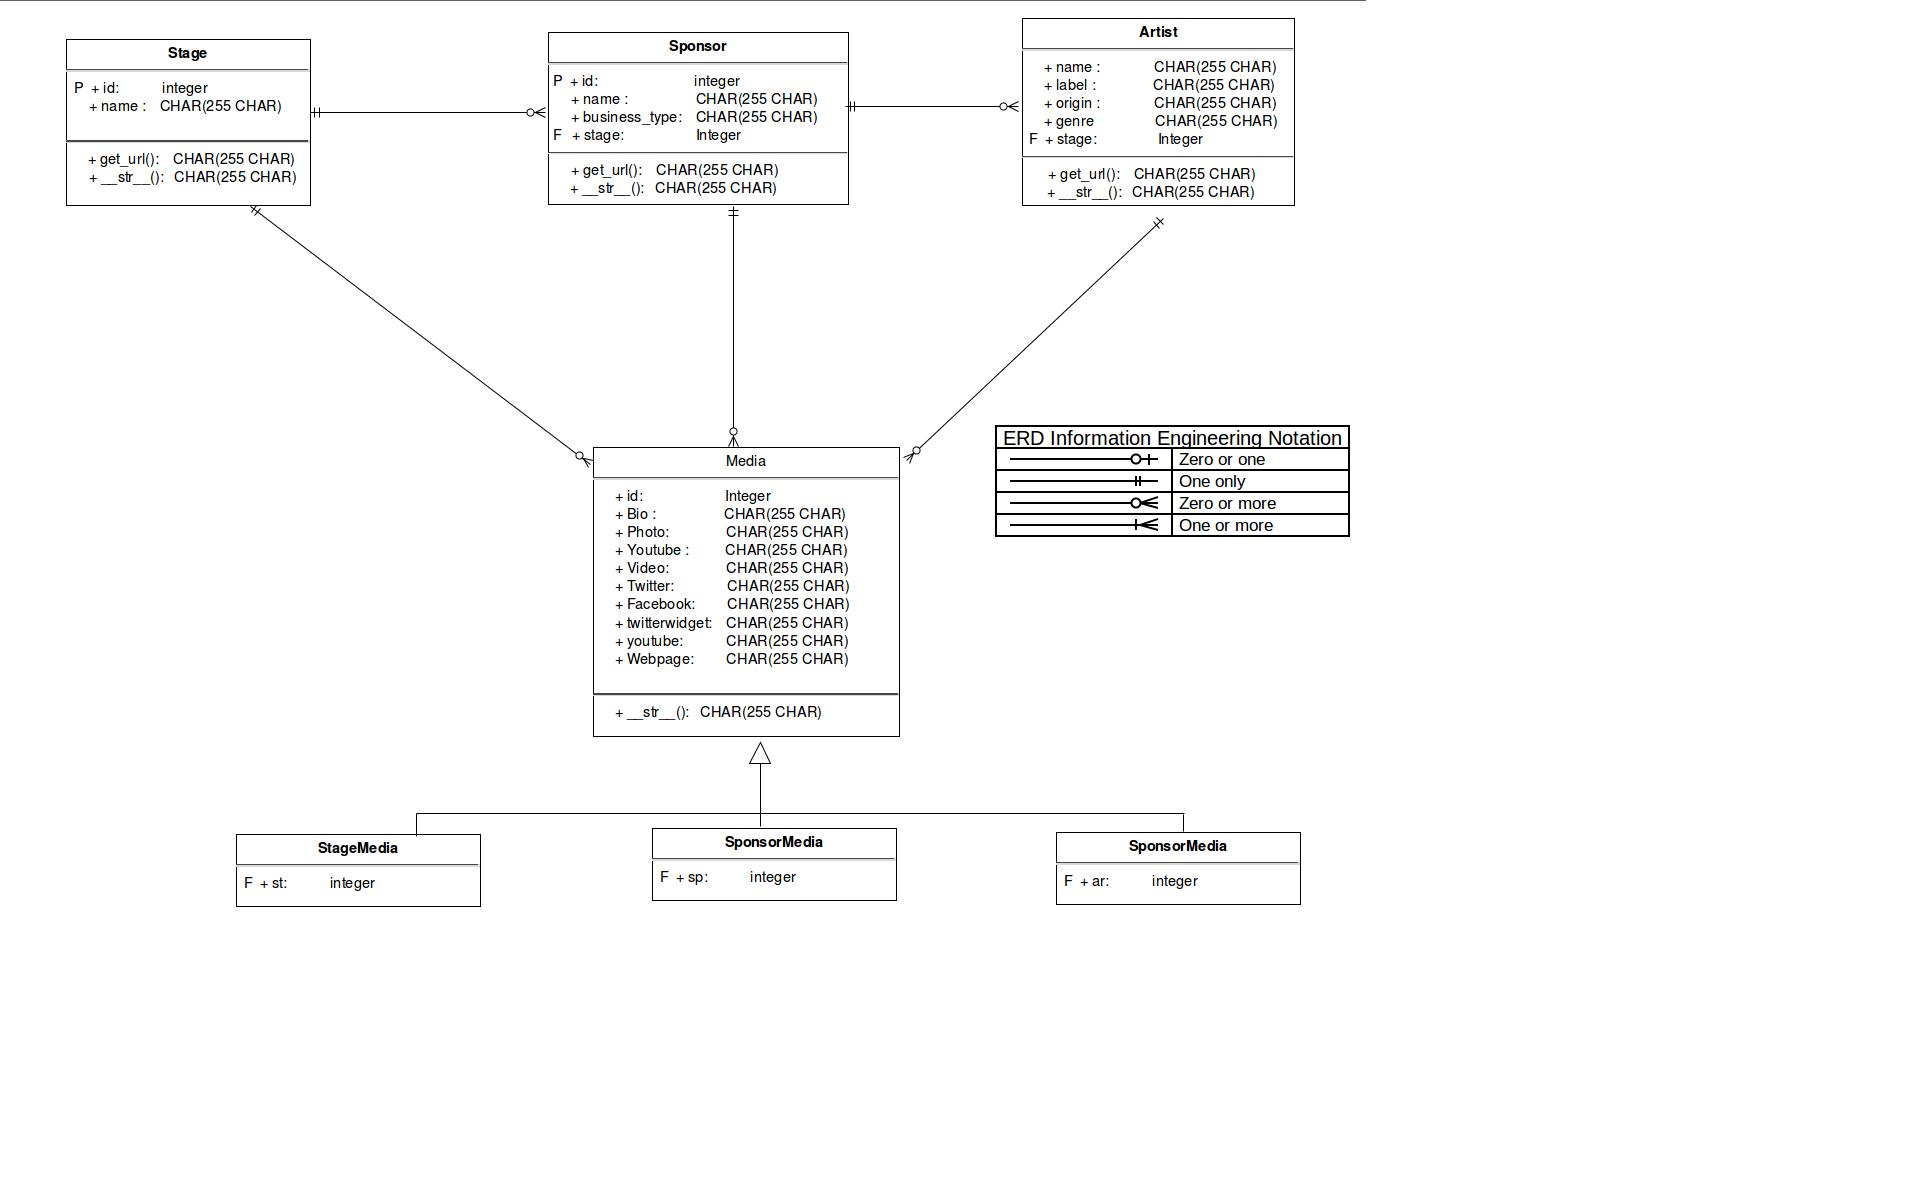
\includegraphics[width=\textwidth]{uml_phase2}
 \caption{The current UML schema depicting the relationships between the Django models. The main three models are Artist, Sponsor, and Stage each of which have an associated Media page.}
\end{figure}

\subsection{Web Pages}
Each web page has basic information about a particular artist, sponsor, or stage involved in the ACL music festival.
All pages will include a navigation bar at the top of their page that will allow the user to go back to the main "splash" page, as well as reach the Artists, Sponsors, and
Stages pages. In future phases we are considering incorporating a search bar inside of the navigation bar, so that the user can search
all categories. Mobile browsers are able to view the webpage correctly and set the height and width to a percentage of the size of the screen.

\subsubsection{Splash Page}
\begin{itemize}
 \item URL: https://theaustinites.pythonanywhere.com/
\end{itemize}

The "splash" page will be the first page a visitor to the site will see. It will provide button style links to all subcategories (Artists,
Sponsors, Stages). Currently the page lists the group name and group members.

\subsubsection{Artists}

\begin{itemize}
 \item URL: https://theaustinites.pythonanywhere.com/artists
\end{itemize}

Artist Pages can be reached from the home page as well as from the Stage or Sponsor pages depending on whether the Artist played on
a Stage that was hosted by a Sponsor.The page currently lists the dynamic web pages for music artists:
\begin{itemize}
 \item Outkast
\end{itemize}

Each Artist page includes the Artist name, an Artist photo, the label, the origin, genre, the sponsor,the stage, a bio,
the official website to the sponsor, a facebook page, a bio, youtube video, youtube channel, and twitter feed.

\subsubsection{Sponsors}

\begin{itemize}
 \item URL: https://theaustinites.pythonanywhere.com/sponsors
\end{itemize}

Sponsor pages can be reached from the home page as well as from the Artist or Stages pages depending on whether the Sponsor hosted a
Stage, and that particular Artist played on that Stage. The page currently lists ACL festival sponsors:
\begin{itemize}
 \item Honda
\end{itemize}
\begin{itemize}
 \item 
\end{itemize}


Each Sponsor page includes the Sponsor name, a sponsor logo, the origin, stage sponsored, the artists playing the stage, the official website to the sponsor,
a facebook page, a bio, youtube video, and twitter feed.

\subsubsection{Stages}

\begin{itemize}
 \item Location: https://theaustinites.pythonanywhere.com/stages/
\end{itemize}

Stage pages can be reached from the Home page (splash) as well as from the Artist or Sponsor pages depending on whether the Sponsor hosted a
Stage, and that particular Artist played on that Stage. The page currently lists the following stages:
\begin{itemize}
 \item 
\end{itemize}
\begin{itemize}
 \item 
\end{itemize}
Each Stage page includes the Stage name, a Stage logo, the artists playing the stage, the official website to the sponsor,
a facebook page, youtube video, and twitter feed.

\subsection{RESTful  API}
The API allows GET requests to the following models: Stages, Sponsors, Artists. The  Members and  Photos models have been deprecated.
The following section will detail the attributes for the modules, and how the server will respond to the GET requests. See 
the Links section below to view the Apiary API.

\subsubsection{Stages}
When a GET is called on $[/stages]$ it will return a JSON representation of all the Stages in the database.  It will be a list of the stages along with their attributes.
When a GET is called on $[/stages/{id}]$ it will return a JSON representation of a single Stage in the database with the given id.  It will list the stage and all of it's attributes
\\
Example of single stage:
\begin{verbatim}
{
         "id": 42,
         "name": "Stage name"
}
\end{verbatim}
\subsubsection{Sponsor}
When a GET is called on $[/sponsors]$ it will return a JSON representation of all the Sponsors in the database.  It will be a list of the sponsors along with their attributes.
When a GET is called on $[/sponsors/{id}]$ it will return a JSON representation of a single Sponsor in the database with the given id.  It will list the sponsor and all of it's attributes
\\
Example of single sponsor response:
\begin{verbatim}
{
        "id": 42,
        "name": "Sponsor name",
        "business_type": "Type of Business",
        "website": "URL of sponsor website",
        "stage": 12
}
\end{verbatim}

\subsubsection{Artist}
When a GET is called on $[/artists]$ it will return a JSON representation of all the Artists in the database.  It will be a list of the artists along with their attributes.
When a GET is called on $[/artists/{id}]$ it will return a JSON representation of a single Artist in the database with the given id.  It will list the artist and all of it's attributes.
\\
Example of single artist:
\begin{verbatim}
{
        "id": 42,
        "name": "Artist name",
        "label": "Label of artist",
        "origin": "Where the artist was from",
        "website": "URL to the artist",
        "genre": "Genre of the artist",
        "stage": 22
}
\end{verbatim}

\subsection{Django Models}
The Django models created represent the entities we believe are essential to modeling the ACL festival.
The following subsections document the attributes and intended functionality of each class instance method. The following sections use
$child$ and $parent$ in the sense of the schema relationship depicted by the UML diagram in Figure 2 and not in the sense of the object oriented inheritance 
(the only object each model extends is models.Model except the Media classes ArtistMedia, SponsorMedia, and StageMedia that inherit from Media). Currently there are a total of six class.

\subsubsection{Artist}
The Artist class represents the current Artists playing on a sponsored stage. All Artists will be a child of some
stage depending on whether they are playing that Stage or not. The entity relation between Sponosor and Artist  The Artist class is implemented using the following:
\begin{verbatim}
attributes:
- name: the name of max length 255 characters.
- label: the artist label with a maximum length of 255 characters.
- origin: the place of origin the artist/group formed with a maximum length of 255 characters.
- genre: the genre associated with the artist. May span more than one. maximum length of 255 characters.
- stage: Foreign Key, integer of type field.

methods:
- get_url(): returns the string "/artists/{id}" . Maximum number of 255 characters.
- __str__(): returns the name string of the artist.Maximum  number of 255 characters
\end{verbatim}


\subsubsection{Sponsor}
The Sponsor class represents the ACL sponsors that sponsor a Stage for the Artist to perform on.
This relationship is expressed using the one-to-many relationship between the Sponsor and the Stage
class. 

The Sponsor class has the following attributes and methods:
\begin{verbatim}
attributes:
- id: Primary Key, integer type field
- name: a character type field with a maximum length of 255 characters
- business_type: a character type field with a maximum length of 255 characters
- stage: Foreign Key, integer of type field

methods:
- get.url(): returns the string "/sponsors/{id}". Maximum number of 255 characters.
- __str__(): returns a string that represents the name of the sponsor.
\end{verbatim}

\subsubsection{Stage}
The Stage class is meant to represent the stage that an Artist will perform on. All stages
have one sponsor. The Stage class extends from the Django models.Models class.

The Stage class has the following attributes and methods:
\begin{verbatim}
attributes:
- id: Primary Key, integer type field
- name: a character type field with a maximum length of 255 characters


methods:
- get.url(): returns the string "/stages/%s/{name}" where name is the stage name.
- __str__(): returns a string that represents the name of the stage
\end{verbatim}

\subsubsection{Media}
The Media class represents all media informaton that is associated with a sponsor, artist, or stage. 

\begin{verbatim}
attributes:
-id: Integer
-bio: A CharField of 255 characters. Biography. 
-photo: A CharField of 255 characters.
-youtube: A CharField of 255 characters. url for Youtube Channel
-video: A CharField of 255 characters.
-twitter: A CharField of 255 characters. url for Twitter
-facebook:A CharField of 255 characters. url for Facebook
-twitterwidget: A CharField of 255 characters.
-webpage: 

methods:
- __str__(): returns the file_name of the photo.
\end{verbatim}

\section{Unit Tests}
The unit tests currently implemented reflect the expected functionality of the django models and database.
Currently we are using the sqlite3 database as a backend. We assume for each function in the set of tests that the state of the database is reset.
There are currently 30 tests with at least 4 tests for each model. The following give descriptions of each model test. 

\subsection{Stage Test}
Total tests: 7
\begin{itemize}
\item test\_create\_empty\_stage: Tests that uninitialized (stateless) Stages can be created.

\item test\_create\_stage : Tests that the $name$ attribute is set correctly when initialized.
 
\item test\_get\_stage: Tests that the $get\_stage$ method returns the Stage instance we saved into the database. Also tests the filtering functionality of setting the id of the instance.

\item test\_stage\_name: Tests the $max\_length$ property of CharField when setting the name of Stage.

\item test\_stage\_url\_1, test\_stage\_url\_2,test\_stage\_url\_3: Tests whether an instance of the desired Stage class 
is saved in the database table and returns the correct $url$ attribute. 
\end{itemize} 

\subsection{Artist Test}
Total tests: 8
\begin{itemize}
\item test\_create\_artist: Tests the Artist instance attributes actually match the given values
that were passed when constructed (including a Stage instance)
 
\item test\_get\_artist: Tests that an instance of Artist can be retrieved from the database with the attributes used to create it.
 
\item test\_empty\_artist: Tests that an IntegrityError is thrown when an Artist instance is saved in the database without setting a ForeignKey.
 
\item test\_empty\_artist\_with\_stage: Tests the default values of an Artist instance with a ForeignKey.
 
\item test\_artist\_name: Tests the $max\_length$ property of CharField when setting the name of Artist.
 
\item test\_artist\_url\_1, test\_artist\_url\_2, test\_artist\_url\_3: Tests that the many-to-one relationship between
Artists and Stages is valid. Also tests the $get\_url$ method returns the correct url according the id of the instance.
\end{itemize} 

\subsection{Sponsor Test} 
Total tests: 6
\begin{itemize}
\item test\_empty\_sponsor: Tests that a Sponsor's default values and ID are set correctly.
 
\item test\_save\_sponsor: Tests that the name matches the passed value given when the Sponsor instance was created.  
 
\item test\_get\_sponsor\_name: Tests the $max\_length$ property of CharField when setting the name of Sponsor.

\item test\_sponsor\_url\_1, \item test\_sponsor\_url\_2: Tests that the $get\_url$ is returned in the proper format.
\end{itemize}


\subsection{API Test} 
The REST API is tested using the django rest framework. The django rest framework has a built in library that allows the tests to mimic API clients that interact with the API.
Currently only GET requests are allowed. Any other request will throw ??? .
\begin{itemize}
\item test\_empty\_sponsor: Tests that a Sponsor's default values and ID are set correctly.
 
\item test\_save\_sponsor: Tests that the name matches the passed value given when the Sponsor instance was created.  
 
\item test\_get\_sponsor\_name: Tests the $max\_length$ property of CharField when setting the name of Sponsor.

\item test\_sponsor\_url\_1, \item test\_sponsor\_url\_2: Tests that the $get\_url$ is returned in the proper format.
\end{itemize}

\section{Expansions}
This section outlines probable features and functions for the next release.
\begin{itemize}

\item More links to more social media accounts (Instagram or SoundCloud) for Artist pages.

\item Stage pages will link to a map of the festival so users can see their location.

\item Sponsor models might also include include an attribute to store business content such as the location of their headquarters, the name of their respective CEOs, stocks, etc.

\item  Tests that will check that the database is correctly populated with its new attributes as well as test all the new methods included.

\item An updated API that will include the option to make put requests so that data can be uploaded using django forms.
\end{itemize}

\subsection{Third Iteration extension}
For the third iteration we are planning to extend the concept of the website to cover years previous to 2014. This would allow 
the user to have more  expressive queries. For example a user might want to know  how many times an artist has played on a stage
or was sponsored by some business, the distribution of businesses by industry that have sponsored certain genres, or simply a 
list of all hip hop artists that have played in ACL from a certain year.
 The propsed change would also enhance the model relationships to become many to many. For example an artist may play on the same stage
 from previous years that were sponsored by different businesses. Also an artist can now play on more than one stage over time. The 
 inclusion of past ACL artists, sponsors, and stages will also allow for more data of each model as a history accumulates. This is our strongest
 reason for the propsed change because the schedule for 2014 has not been published yet and it may take some time before it does get published. Implementing this
 proposal will address our curent problem. We plan on including timelines for each Artist, Sponsor, and Stage page to take advantage of this extension.
 
\section{Links}

\begin{itemize}
 \item Home Page: https://theaustinites.pythonanywhere.com/
 \item Apiary API: http://docs.aclprojectapi.apiary.io/
 \item Github: https://github.com/sandan/cs373-idb
 \item http://www.aclfestival.com/
\end{itemize}

\end{document}